\documentclass[a4paper, 12pt]{article}

\usepackage[left = 3cm, top = 3cm, bottom = 3cm, right = 2cm]{geometry}
\usepackage{graphicx}
\usepackage[spanish,es-tabla]{babel} % Idioma español con tablas
\usepackage{amsmath}
\usepackage{amssymb}
\usepackage{amsfonts}
\usepackage[utf8]{inputenc}         % Para escribir en castellano
\usepackage[T1]{fontenc}
\usepackage{color}
\usepackage{alltt}
\usepackage{times}
\usepackage{setspace}  % Usado para doble espacio, espacio y medio y espacio simple
\usepackage{booktabs}         % Para formar tablas
%\usepackage{longtable}       % Usado para diseñar grandes tablas.
\usepackage[round]{natbib} 
\bibliographystyle{apalike}
\usepackage{hyperref}


\begin{document}



\begin{center}
%\onehalfspace  \doublespacing  \singlespace
\Large {Comportamiento y Características de los polinomios AKS con exponente compuesto \(n\in \mathbb{N}\)} \\
\vskip 0.2cm
 \end{center}
\vskip 1cm
\begin{center}
\section*{{\large{Jahir G. Medina Lopez}}\\ {\it \small{jahir.medina@unitru.edu.pe}\\ \small{ Escuela de Informática - UNT, Trujillo, Perú.}} }
\end{center}

\begin{abstract}
En este artículo se estudia el comportamiento de los polinomios AKS de exponente generatriz natural compuesto.
Se plantea un método de factorización para números semiprimos, su vinculación con los números de Carmichael, además de características relevantes a su comportamiento geométrico en el plano cartesiano.


\vskip 0.3cm
\hspace*{-0.6cm}{\bf Palabras claves:} polinomio AKS, números semiprimos, prueba de primalidad, números de Carmichael, números compuestos, factorización
\end{abstract}

\section{Introducción}
Los polinomios AKS (en honor a las siglas de sus autores), necesarios para la demostración del algoritmo AKS \citep{AKS} tienen un valor importante en el campo de la teoría de números, al ser el primer algoritmo determinista para prueba de primalidad en tiempo polinomial , significando su pertenencia al conjunto de problemas tipo P , lo cual implica su resolución en un \textit{tiempo aceptable} \citep[Lectura 1]{pteory} , sin embargo la primera aparición de estos polinomios data de 1999, en un trabajo preliminar de uno de los autores del algoritmo AKS, en el artículo \textit{Primality and Identity Testing via Chinese Remaindering} \citep{preAKS}, que es de donde el presente artículo toma su definición:
\[ \mathcal{P}_{n}(z) = (1 + z)^{n} - 1 - z^{n}  \]
\
El trabajo realizado aquí se enfoca solo en el polinomio descrito originalmente y su comportamiento cuando su exponente generatriz es un numero compuesto natural, es valido aclarar que la denominación \textbf{polinomios AKS}\ nace de su forma general:
\[ \mathcal{P}_{n}(z) = (a + z)^{n} - a - z^{n} \]
\[\text{donde: } \gcd(n,a) = 1\]
Tal como se puede observar, el polinomio AKS es un tipo de binomio con la cualidad de tener por exponente un numero $n$ tal que este es \textbf{coprimo} con uno de los elementos indeterminados($a$).

Este artículo no enfocara su análisis desde el punto de vista estrictamente polinomial,usando en mayor medida los coeficientes \citep{biPas}, haciendo empleo del triángulo de pascal y las definiciones combinatorias dadas por newton para los binomios \citep{binew}.
En el conjunto de los números compuesto, existen dos subconjuntos: los semiprimos y los Carmichael, estos números presentan comportamientos específicamente interesantes al ser relacionados con los polinomios AKS.

Como nota final, se debe aclarar el presente trabajo aun esta en proceso, por lo que muchas demostraciones se encuentran pendientes; para respaldar las conclusiones (donde sea necesario) se usar los datos obtenidos mediante calculo computacional.
\pagebreak
\section{Trabajos relacionados}\ \\
\
\subsection{Binomio de Newton y Coeficiente Binomial}
Considerando la definición de \textbf{Binomio de Newton} a partir de el Lema 2 \citep*[pag 11]{binew}

\[ (x + y)^{n} = \sum_{k=0}^{n}\binom{n}{k} x^{n-k} y^{k} \]
donde $x \land y \in \mathbb{R}$ y $n \in \mathbb{N}$ , ademas $\binom{n}{k}$ se define como:\\
\begin{equation}\label{binomio}
 \binom{n}{k} = \frac{n!}{k!(n-k)!} 
\end{equation}
denominado \textbf{coeficiente binomial} , a partir del cual se puede completar la definición del \textbf{triangulo de pascal} \citep[pag 4]{biPas} , definiéndose como \textbf{el triángulo generado al sumar los dos elementos inmediatamente superiores}, creando un arreglo triangular:
\begin{figure}[h]
	\centering
	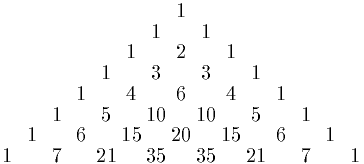
\includegraphics[width=0.3\linewidth, height=0.1\textheight]{Pascal_triangle_small}
	\caption[Triangulo de Pascal]{Primeras 7 filas correlativas con los coeficientes de $(x+1)^{n}$ estando $n \in [0,7]$ }
	\small{fuente: Re-diseño \citep[pag. 11]{littleFermatBook}}
	\label{fig:pascaltrianglesmall}
\end{figure} 

\subsubsection{Propiedades}

\begin{itemize}
	\item La suma de elementos de la fila $n$ es igual a $n^{n}$
		
		\begin{equation}\label{sumPas}
			\sum_{k=0}^{n}\binom{n}{k} = 2^{n} 
		\end{equation}
	\item Los elementos del triángulo poseen simetría axial derivado de la propiedad de los coeficientes
	
		\begin{equation}\label{simetri}
			\binom{n}{i} = \binom{n}{n-i}
		\end{equation}
	
	\item De \ref{sumPas} y \ref{simetri} se puede describir la suma de elementos de una fila como:	
		 \begin{equation}\label{par}
			 2(\sum_{i = 0}^{\frac{n}{2} -1}\binom{n}{i}) + \binom{n}{\frac{n}{2}} = 2^{n}
			 \iff n \equiv 0 (mod2)
		 \end{equation}
		 
		 \begin{equation}\label{inpar}
		 2(\sum_{i = 0}^{\frac{n-1}{2}}\binom{n}{i})= 2^{n}
		 \iff n \equiv 1 (mod2)
		 \end{equation}
		
		
\end{itemize}

\subsection{Polinomio AKS}\ \\
\
Definiéndose la familia de polinomios AKS como todo polinomio de la forma:
\[ \mathcal{P}_{n}(z) = (a + z)^{n} - a - z^{n} \]
\[\text{donde: } \gcd(n,a) = 1\]
\[n \land a \in \mathbb{N}\]
y el polinomio AKS original \citep[pag. 3]{preAKS} 
\begin{equation}\label{aksorig}
 \mathcal{P}_{n}(z) = (1 + z)^{n} - 1 - z^{n} 
\end{equation}
reescribiéndolo de la forma:
\[ \mathcal{P}_{n}(z) = \sum_{j=1}^{n-1}\binom{n}{j} z^{j} \]
y a su término general de la forma:
\[ t_{j} = \binom{n}{j} z^{j} \]
donde $\binom{n}{j}$ es un \textbf{coeficiente entero} ,pues $n \land j \in \mathbb{N}$.\\
\ \\
Además $z \in \mathbb{X}$, $\mathbb{X}$ es un \textbf{grupo} donde $z$ representa un elemento cualquiera, denominado \emph{indeterminada} \citep[pag. 100]{indeterminate}.
\ \\
\subsubsection{Caso Particular}
\ \\
Sea $n$ un \textbf{numero primo} definido en $\mathbb{N}$ y usando el lema 3.1 \cite[pag. 4]{AKS}
cumple que:
\[ \mathcal{P}_{n}(z) \equiv0(\mathbf{mod}\ n) \rightarrow \mathcal{P}_{n}(z)\  \text{es identicamente nulo} \]
\\
\
\subsection{Definiciones Adicionales}
\begin{itemize}
	\item Se define un numero compuesto como semiprimo, si es de la forma:
	\[n = p \cdot q\]
	\[p \land q \  \text{son primos} \]
\end{itemize}
\section{Propuesta}
\subsection{Definición de un Triángulo Modular AKS}
\ \\
\
Presentando la idea de un \textbf{Triangulo de Pascal Modular del Polinomio AKS} o \textbf{AKS-MPT}, definido como:

\begin{verse}
	El arreglo triangular que se forma al sustituir los elementos clásicos de un triángulo de pascal (coeficientes binomiales de $(x+1)^{n}$) por los coeficientes del \textbf{polinomio AKS original} y aplicando sobre todos ellos la \emph{operación modulo con respecto a su número de fila}.
\end{verse}
\ \\
De esta definición y su sucesivo cálculo obtiene dos tipos de filas en el triángulo:
\begin{itemize}
	\item Una fila de $0$'s cuando $n$ es \textbf{primo}
	\item Una fila con valores \textbf{enteros} menores a $n$ , cuando $n$ es \textbf{compuesto}
\end{itemize}\

\begin{figure}[h!]
	\centering
	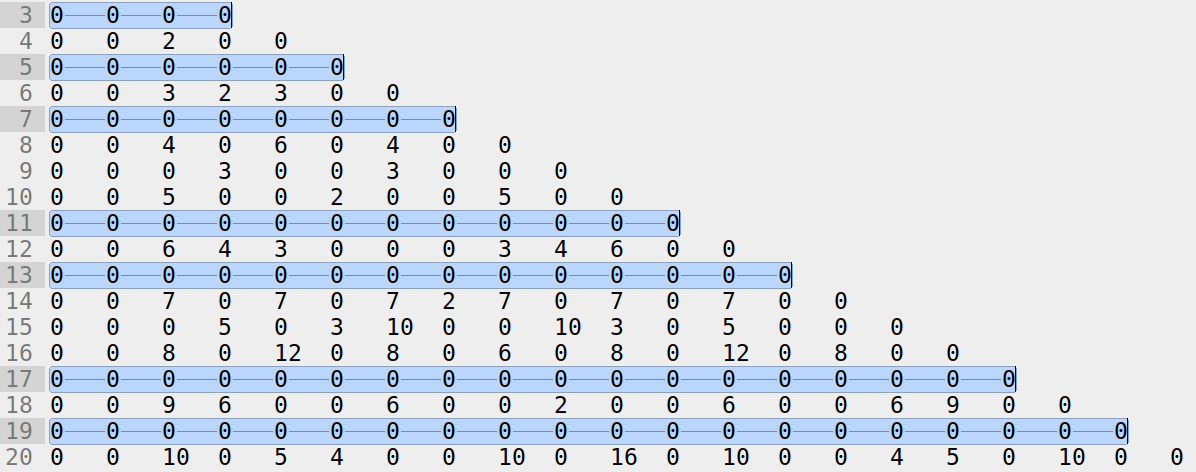
\includegraphics[width=0.7\linewidth, height=0.4\linewidth]{AKS-MPT}
	\caption[AKS - MPT]{Triangulo generado desde la fila 3 hasta la fila 20, resaltado en azul las filas de orden primo}
	\small{fuente: Propio}
	\label{fig:aks-mpt}
\end{figure}
\ \\
De manera formal, un elemento cualquiera de una fila cualquiera del \textbf{AKS-MPT} se define:

\begin{equation}\label{aks-mptGen}
t_{j}(n) = \binom{n}{j}(\mathbf{mod}\ n)
\end{equation}
\[n \land j \in \mathbb{N}\]
De la definición original para el \textbf{polinomio AKS} se sabe que:
\begin{itemize}
	\item si $n$ es \textbf{primo}
	\begin{equation}\label{primeAKSROW}
	t_{j}(n) = 0 \lor \binom{n}{j} \equiv 0(\mathbf{mod}\ n)
	\end{equation}
	\item si $n$ es \textbf{compuesto}
	\begin{equation}\label{compositeAKSROW}
	\exists ! \ \  t_{j}(n) \neq 0 \lor \binom{n}{j} \equiv m(\mathbf{mod}\ n)
	\end{equation}
	donde $m \in [1,n-1]$
\end{itemize}\

\subsection{Operaciones Asociadas y Características de AKS-MPT}

\subsubsection{Número de Elementos}

Si en un triángulo de pascal normal, el número de elementos es siempre igual al\textit{ número de orden de la fila aumentado en una unidad}, en el \textbf{AKS-MPT}, este número varia a causa de las características de su polinomio generatriz (definición \ref{aksorig}) , de donde se puede observar pierde el primer y último elemento los cuales son la unidad, adicionalmente en la definición \ref{aks-mptGen} se observa que cuando $j = 1$:

\begin{equation}\label{nelement}
\binom{n}{1}(\mathbf{mod}\ n) = \binom{n}{n-1}(\mathbf{mod}\ n) = n(\mathbf{mod}\ n) = 0
\end{equation}
\ \\
Por lo tanto el número de \textbf{elementos significativos} (aparente) es:
\[(n + 1) - 4\]
\[n - 3\]

pero por el comportamiento combinatorio de los coeficientes binomiales, puede existir algún coeficiente que no se encuentre en los extremos que cumpla:
\[ \binom{n}{j} = 0 (\mathbf{mod}\ n) \]
definiendo asi, que el número de elementos es:
\begin{equation}\label{elements}
		\#nro \leq n - 3
\end{equation}

\subsubsection{Características de los Coeficientes}

mediante un cálculo asistido por computadora de las primeras $7000$ filas del \textbf{AKS-MPT} se observa que:

\begin{equation}\label{composite}
j\cdotp(t_{j}(n)) \equiv 0 (\mathbf{mod}\ n) \ ,\  \forall \ n \ \text{compuesto}
\end{equation}


\ \\
\
\textbf{Sin embargo un caso importante ocurre cuando:}

\begin{center}
	sea $n$ un \textbf{numero compuesto semiprimo} y $t_{j}(n)$ un elemento de la fila $n$ del AKS-MPT, se cumple que si $t_{j}(n)$ es el \textbf{primer número no nulo desde la izquierda} en su fila correspondiente del AKS-MPT entonces:
	
	\begin{equation}\label{semiprimes}
	j\cdotp t_{j}(n) = n 
	\end{equation}
siendo $j$ el menor factor primo y $t_{j}(n)$ el mayor
\end{center}


\subsubsection{Suma de elementos AKS-MPT}

 Para un triángulo de Pascal Común, modificando \ref{sumPas} usando \ref{nelement}:
	
	\[\sum_{k=2}^{n-2}\binom{n}{k} + \binom{n}{1} + \binom{n}{n-1} + 1 + 1  = 2^{n}\]
	\[\sum_{k=2}^{n-2}\binom{n}{k} + 2(n) + 2  = 2^{n}\]
	\begin{equation}\label{mptSum}
			 \sum_{k=2}^{n-2}\binom{n}{k} = 2^{n} -2 (n) - 2
	\end{equation}

Usando la definición \ref{aks-mptGen} y la propiedad distributiva respecto a la suma del módulo:
	
	\[ 	(\sum_{i = 2}^{n-2}\binom{n}{j}(\mathbf{mod}\ n))(\mathbf{mod}\ n)  = (2^{n} -2(n) - 2)(\mathbf{mod}\ n) \]
	
	\begin{equation}\label{sumAKSMPT}
		\sum_{i = 2}^{n-2}\binom{n}{j}(\mathbf{mod}\ n) \equiv (2^{n} -2(n) - 2)(\mathbf{mod}\ n)
	\end{equation}

cuando $n$ es primo todos los elementos son 0 (def. \ref{primeAKSROW})
	
	\[ \sum_{i = 2}^{n-2}\binom{n}{j}(\mathbf{mod}\ n) = 0 \]
	\[ (2^{n} -2(n) - 2)(\mathbf{mod}\ n) = 0 \]
	\begin{equation}\label{primaltyTest}
	\Rightarrow  (2^{n} -2(n) - 2) \equiv 0 (\mathbf{mod}\ n)
	\end{equation}
	
cuando $n$ es primo.

\subsection{Números de Carmichael}

En la definición \ref{primaltyTest} se puede observar una ecuación relativamente semejante al pequeño teorema de Fermat para pruebas de primalidad \citep[pag. 97]{littleFermatBook}

 \begin{equation}\label{littleFermateq}
 a^{n-1} = 1 (\mathbf{mod}\ n)
 \end{equation}
cuando $n$ es primo.
\ \\
Siendo $a \land n$ \textbf{coprimos} , esto significa que $\gcd(a,n) = 1$ y dado que en la ecuación \ref{primaltyTest} se sabe $n$ es primo al igual que $2$ ( para evitar ambigüedades $n \geq 3$, esto no afecta las definiciones ya dadas)
se deduce que $\gcd(2,n)$ siempre será $1$ y por tanto coprimos.
\pagebreak
\ \\
Los números de Carmichael se definen como todo numero $n$ que cumple la ecuación \ref{littleFermateq} sin ser primo \citep{carmichaelNum}, se sabe que estos números son relativamente escasos en comparación con los números primos.

En concordancia con el calculo asistido por computadora de las primeras $7000$ filas del \textbf{AKS-MPT} se puede contrastar que los \textbf{números de Carmichael} menores a $7000$

\[561, 1105, 1729, 2465, 2821, 6601\]

tienen una coincidencia del\textbf{ $100\%$} de fallos al ser estos probados en la ecuación \ref{primaltyTest}, mientras que para los demás valores actúan de la forma esperada. Por consiguiente es valido inferir que la ecuación \ref{primaltyTest} tiene similar comportamiento matemático en su rango que \textbf{el pequeño teorema de Fermat} [\ref{littleFermateq}].

\subsubsection{Filas AKS-MPT de orden Carmichael}\label{carmichaelDef}

En las primeras $7000$ filas, solo aparecen $6$ polinomios AKS de exponen $n$ siendo $n$ un numero de Carmichael; usando AKS-MPT se obtiene los polinomios (por comprensión):
\begin{itemize}
	\item $n = 561$
	\[ \sum_{k=2}^{599}\binom{561}{k} z^{k}\]
	\item $n = 1105$
	\[ \sum_{k=2}^{1103}\binom{1105}{k} z^{k}\]
	\item $n = 1729$
	\[ \sum_{k=2}^{1727}\binom{1729}{k} z^{k}\]
	\item $n = 2465$
	\[ \sum_{k=2}^{2463}\binom{2465}{k} z^{k}\]
	\item $n = 2821$
	\[ \sum_{k=2}^{2819}\binom{2821}{k} z^{k}\]
	\item $n = 6601$
	\[ \sum_{k=2}^{6599}\binom{6601}{k} z^{k}\]
\end{itemize}

Por una corazonada se calculó el $\gcd(n,\binom{n}{k})$ para todos sus coeficientes, con la idea de que dichos coeficientes serian coprimos de $n$, sin embargo, se observo que si bien no eran coprimos tenían la siguiente característica :
\begin{equation}\label{carmichaelN}
	n = \gcd(n,t_{k}(n))\cdot k
\end{equation}
pero también se observo que:
\[ \gcd(n,t_{k}(n)) = t_{k}(n) \]
por lo que para el caso de las filas AKS-MPT de orden Carmichael la ecuación \ref{carmichaelN} se simplifica a:
\begin{equation}\label{carmichaelGen}
 n = t_{k}(n) \cdot k 
\end{equation}
resultado similar a si el exponente fuese semiprimo (ecuación \ref{semiprimes})
\section{Resultados}
\subsection{Computacionales}
En la sección anterior se revisó y determino el comportamiento aritmético del polinomio AKS con respecto a sus coeficientes y los números de Carmichael, en esta parte, se mostrará el comportamiento geométrico.
\subsubsection{Polinomio AKS General con $\mathbb{X} = \mathbb{R}$}
\begin{figure}[h!]
	\centering
	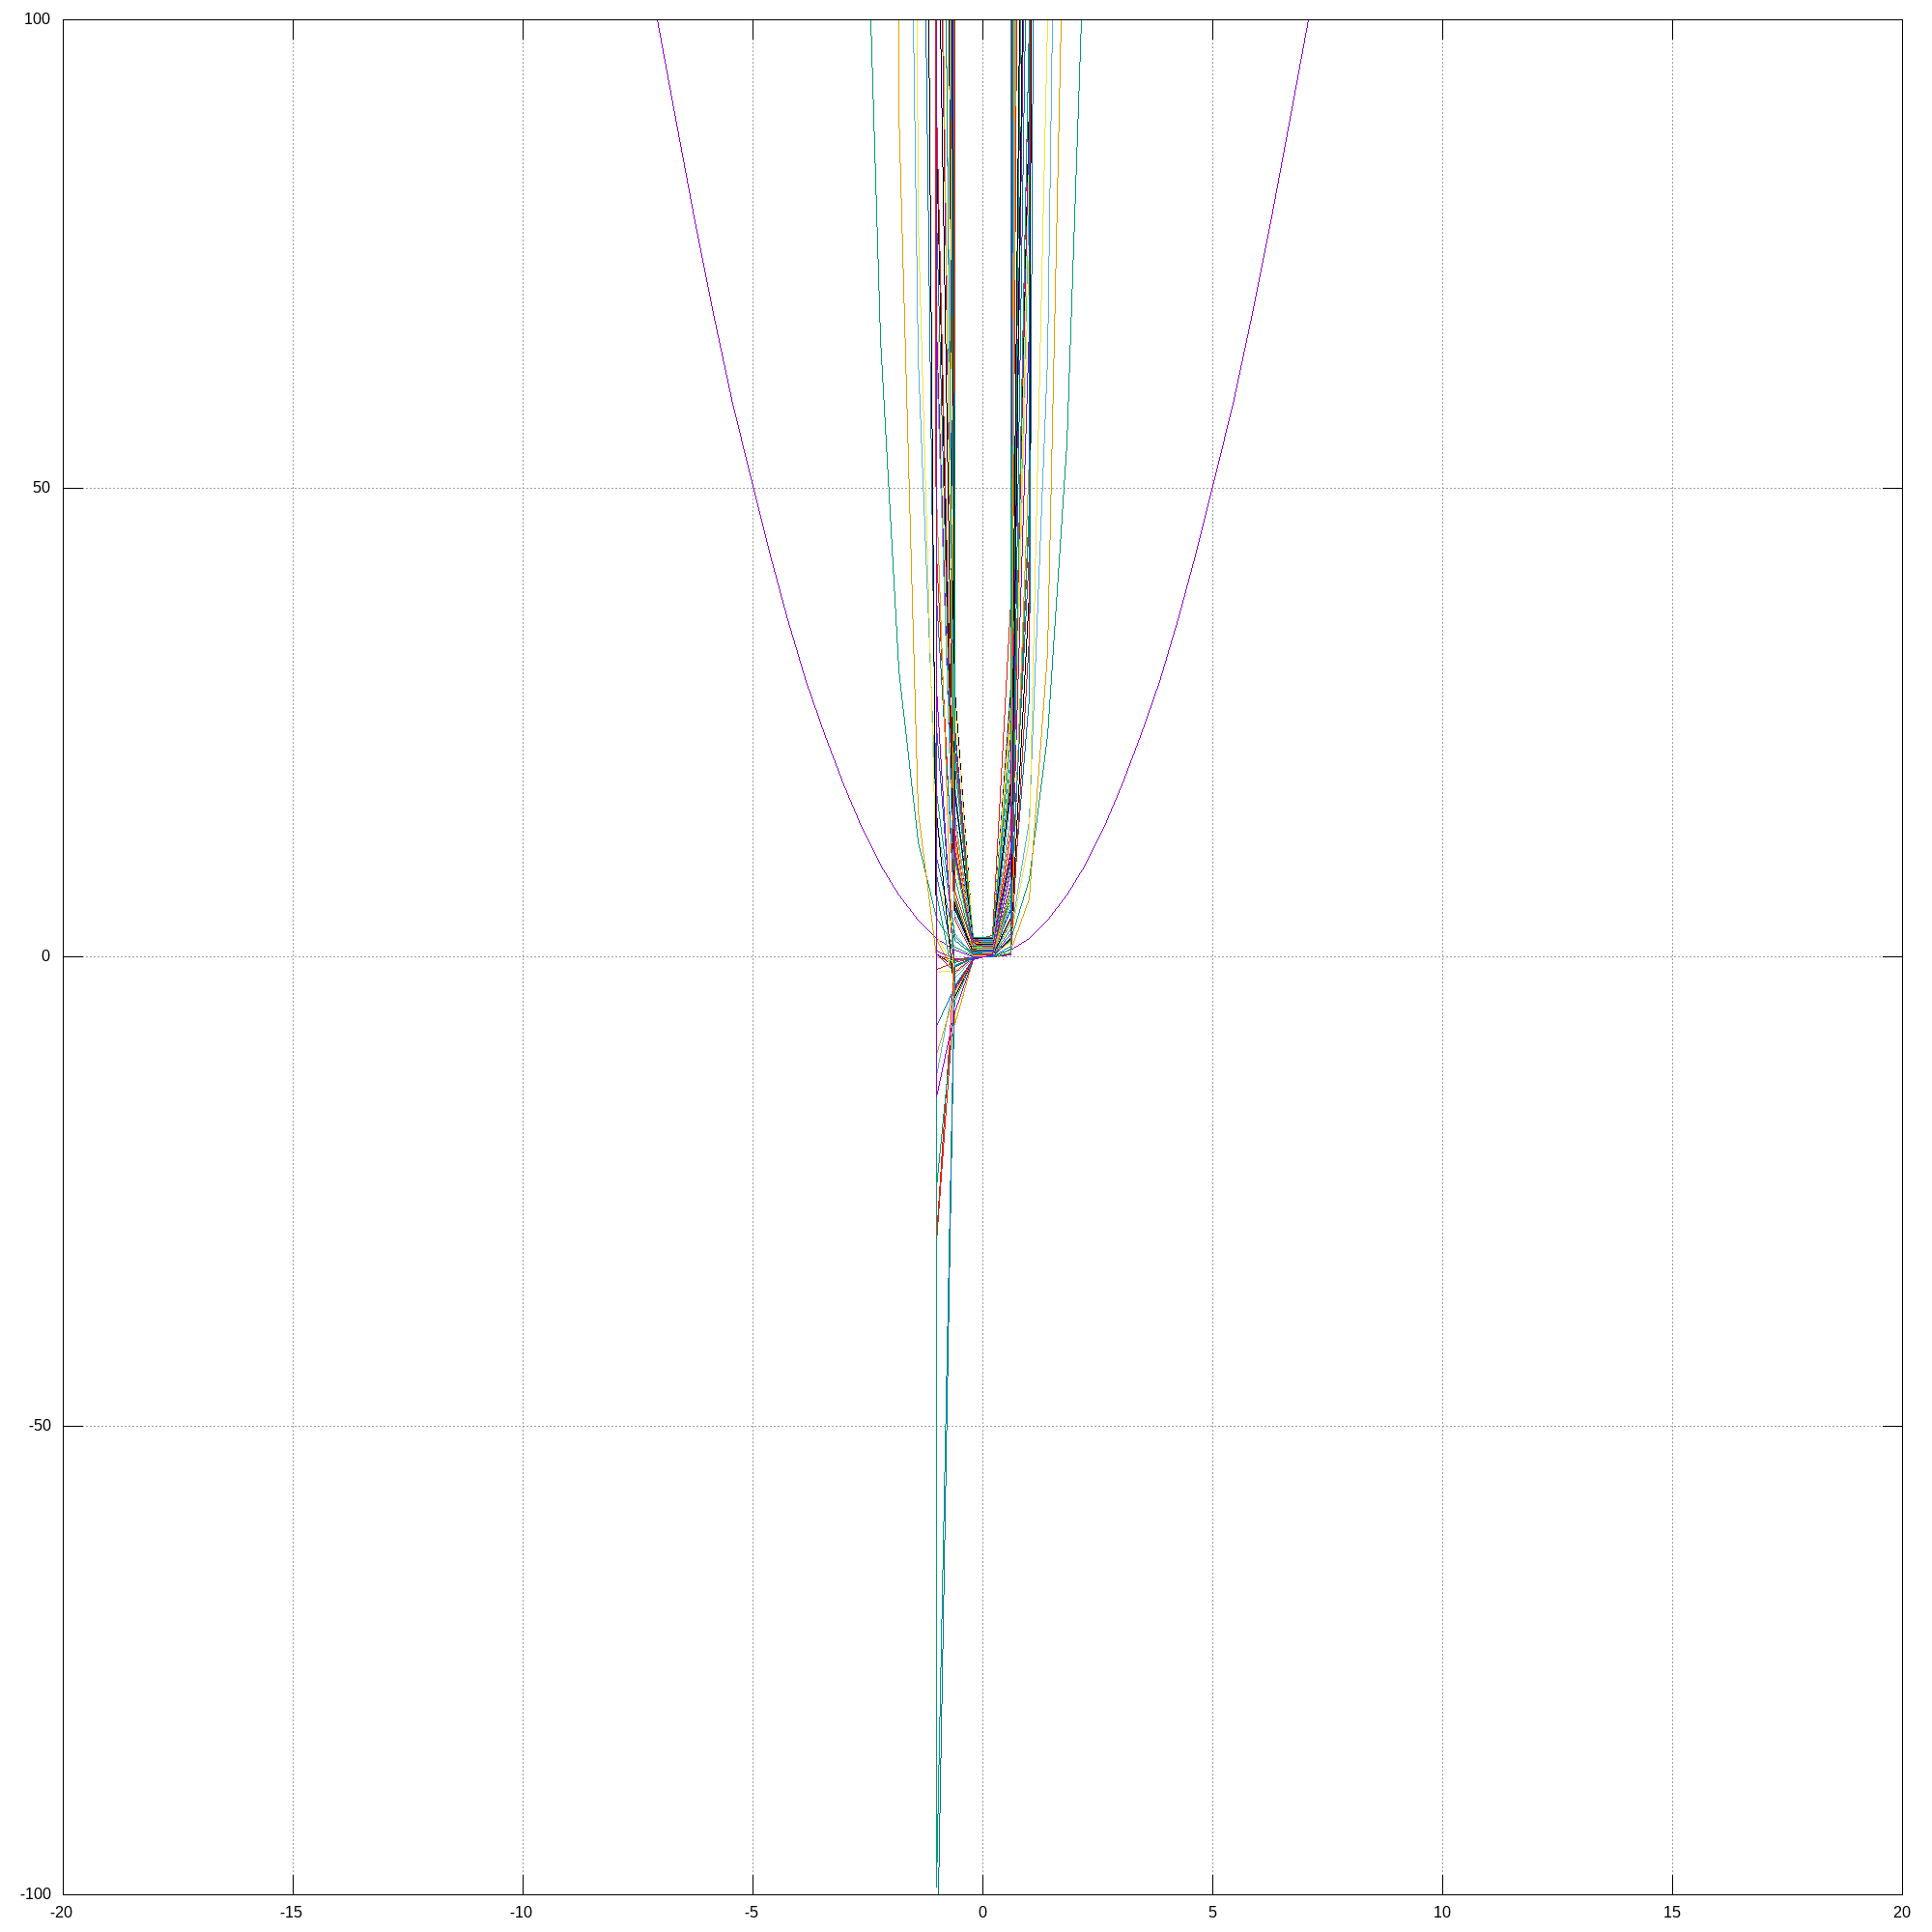
\includegraphics[width=0.9\linewidth, height=0.7\linewidth]{nonAKSp}
	\caption[Polinomios AKS $(x + 1)^n$]{Grafica de los polinomios AKS cuando $n \in [3,100]$ y $x \in \mathbb{R}$}
	\small{fuente: Propio}
	\label{fig:nonaksp}
\end{figure}

En esta imagen se puede observar que cuando un polinomio AKS se opera sobre los $\mathbb{R}$ su comportamiento geométrico no difiere en nada de los binomios comunes \cite{}

\pagebreak

\subsubsection{Polinomio AKS-MPT con $\mathbb{X} = \mathbb{R}$}
En este caso en particular, donde la operación $ (\mathbf{mod}\ n) $ resulta relevante, pues es quien aparentemente genera la tendencia de $\mathcal{P}_{n}(z)$  a acumularse cerca del eje $x$ , en otras palabras, tender hacia $0$.

\begin{figure}[h!]
	\centering
	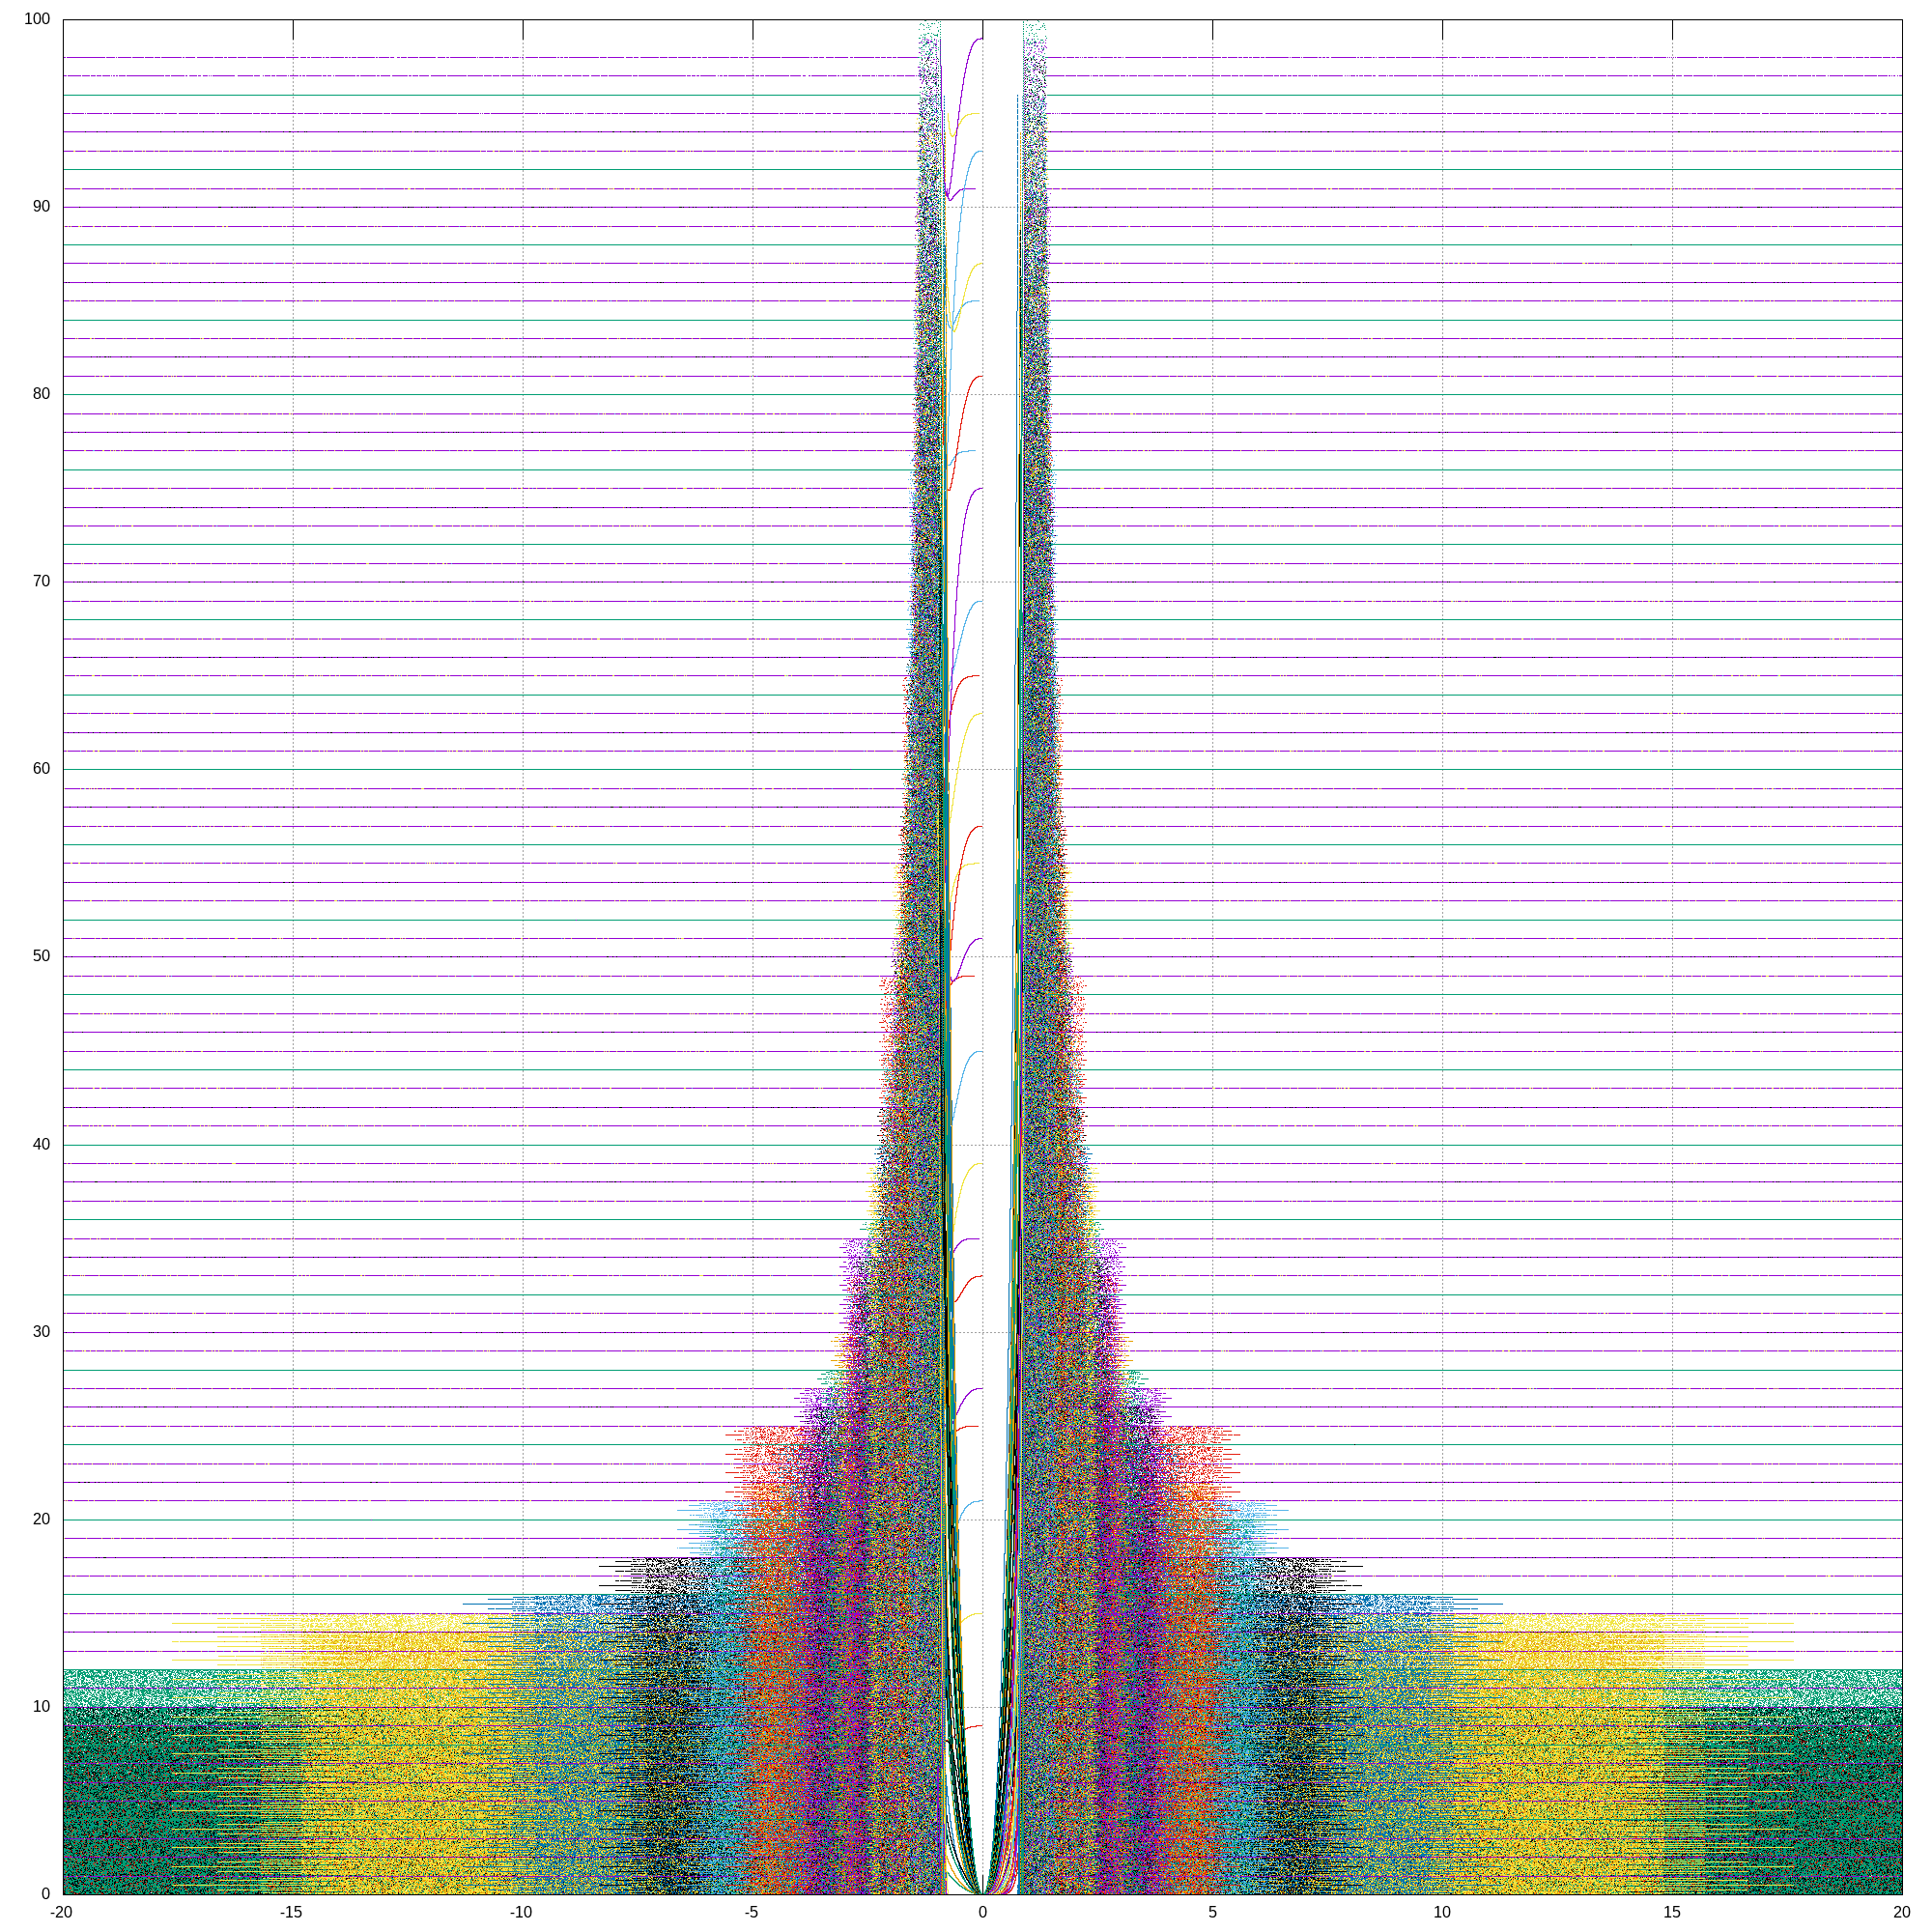
\includegraphics[width=0.8\linewidth, height=0.4\textheight]{plot}
	\caption[AKS-MPT sobre indeterminada $\mathbb{R}$]{Los coeficientes generados por el AKS-MPT en forma polinomial $x \in [-20,20] \land n \in [3,100]$}
	\small{fuente: Propio}
	\label{fig:nonaksmodp}
\end{figure}

Este comportamiento acumulativo puede deberse a la característica de sus coeficientes descrita por la definición \ref{composite}, de manera que al sustituirse el valor indeterminado solo queda de resto $x^{j} (\mathbf{mod}\ n)$.
Dado que esta expresión se puede escribir como:
\begin{equation}\label{resGraph}
	x^{j} = l (\mathbf{mod}\ n)
\end{equation}
estando $l \in \langle0,n\rangle$ , resultado de extender la operación $\mathbf{mod}$ al grupo de los $\mathbb{R}$ ,trabajando solo con la parte entera y dejando la parte decimal intacta.
Ya que en $a' \in [a,a+1]$ la operación $\mathbf{mod}$ extendida se limita a
$a' \in [a (\mathbf{mod\ n}),a+1(\mathbf{mod\ n})]$ dejando los valores no enteros de la forma
\begin{equation}\label{sigma}
	a' = a (\mathbf{mod\ n}) + \sigma
\end{equation}
\[\sigma \in \langle0,1\rangle \]
si $\sigma$ es elevando a la potencia $j$ el resultado sigue perteneciendo al intervalo $ \langle0,1\rangle$, por consiguiente se puede asumir que solo resulta relevante estudiar la parte de entera residual obtenida en la ecuación \ref{resGraph}.
Del gráfico y la definición \ref{sigma} podemos manifestar que el resultado de trabajar sobre los reales tiene relevancia solo la parte entera, la cual es, quien en última instancia se empieza a acumular cerca del eje $x$ o del valor $0$ en $y$.
Un explicación mas detallada requeriría cálculos con rangos superiores a $[-20,20]$ y la demostración analítica de esta convergencia.
\subsection{Detalles de Resultados}
Dado que los resultados computacionales contienen 7000 columnas y habiendo 4 diferentes tipos, se dejara un enlace hacia \textbf{github} , de donde se podrá descargar los datos completos y el script usado para su generación:
\ \\
\
enlace:
\href{https://github.com/coituselpingo/Comportamiento-y-Caracteristicas-de-los-polinomios-AKS-con-exponente-compuesto-n-N.git}{\textbf{Comportamiento-y-Caracteristicas-de-los-polinomios-AKS-con-exponente-compuesto-n-N.git}} 

\subsubsection{Script}
Amen de no alargar el articulo de forma innecesaria, no se pondrá el script directamente, solo una descripción técnica.
El script desarrollado para los cálculos se encuentra escrito en \textbf{python} ,para la versión $2.7.13$,; no se empleó ningún algoritmo especial, sin embargo, para el cálculo de las filas se aposto por operaciones secuenciales que ocupen memoria y no potencia de cálculo.

Como se describe anteriormente, el cálculo de los coeficientes de los polinomios y elementos del AKS-MPT no emplea el cálculo combinatorio al ser excesivamente demandante la recursión factorial; sin embargo, si se emplea la técnica original del triángulo de pascal de sumas sucesivas.
\subsubsection{Tablas de Resultados}
\begin{itemize}
	\item Definiciones \ref{primeAKSROW} y \ref{compositeAKSROW} basadas en el archivo
		\href{https://github.com/coituselpingo/Comportamiento-y-Caracteristicas-de-los-polinomios-AKS-con-exponente-compuesto-n-N/blob/master/patron de coeficientes.dat}{\textbf{patrón de coeficientes.dat}}
	\item Patrón usado para definir la ecuación \ref{carmichaelGen} y Parte \ref{carmichaelDef} revisar los archivos
		\href{https://github.com/coituselpingo/Comportamiento-y-Caracteristicas-de-los-polinomios-AKS-con-exponente-compuesto-n-N/blob/master/carmichael_test.dat}{\textbf{carmichael test.dat}} y \href{https://github.com/coituselpingo/Comportamiento-y-Caracteristicas-de-los-polinomios-AKS-con-exponente-compuesto-n-N/blob/master/carmichael_polinomios.dat}{\textbf{carmichael polinomios.dat}}
	\item Grafica de polinomios AKS (figura \ref{fig:nonaksp}) sobre los $\mathbb{R}$ generada desde el archivo \href{https://github.com/coituselpingo/Comportamiento-y-Caracteristicas-de-los-polinomios-AKS-con-exponente-compuesto-n-N/blob/master/polinomios Generales.plot}{\textbf{polinomios Generales.plot}}
\end{itemize}
 
\subsection{Teóricos}
El presente artículo trata a todas sus definiciones, ecuaciones y suposiciones como verdaderas, mas no por tanto deben ser tomadas como tales, el trabajo aquí presentado es de carácter descriptivo más que analítico, siendo esta una versión inicial se espera en futuras versiones incluir definiciones y demostraciones completamente analíticas que den un respaldo solido a los cálculos obtenidos vía asistencia computacional.




\section{Conclusiones y trabajos futuros}
\subsection{Conclusiones}

El polinomio AKS presenta un gran campo de estudio, no solo para la teoría de números, sino también para la criptografía, en donde se puede emplear en la definición \ref{semiprimes} para factorizar los números RSA \cite[pag. 5 sección V]{RSA}, caracterizados por ser semiprimos, sin tener que recurrir las divisiones sucesivas.
Para este fin, el presente artículo deja a disposición el script usado para generar las $n$ filas del AKS-MPT, si este $n$ fuese un \textbf{número RSA} la factorización quedaría inmediatamente determinada por:
\[ j\cdot t_{j}(n) = n  \]
De ser requerido $j$ puede ser obtenido de forma aleatoria y recurri a la formula con la forma:
\[ j \cdot \binom{n}{j} = n\]

Aunque esta aplicación resulta en un consumo exagerado de recursos computacionales (sumas sucesivas)  se puede optimizar si se analiza con mayor detalle los patrones que oculta los polinomios AKS con exponente compuesto $n \in \mathbb{N}$, el método empleado aquí resulta especialmente favorable durante estudios descriptivos, ya que aun no ofrece directamente ninguna demostración analítica propiamente dicha, el AKS-MPT posee ventaja sobre los métodos polinomiales de análisis cuando se trata de ubicar patrones usando solo la intuición.

 
\subsection{Trabajos futuros}

Se sugiere revisar el caso de los exponentes $n$ que sean números de Carmichael, su relativa relación con el pequeño teorema de Fermat puede resultar en la obtención de nuevos patrones.

Finalmente se recomienda re-calcular y re-graficar los valores para los polinomios AKS sobre el grupo de los complejos, quizás el comportamiento con tendencia a acumularse hacia $0$ resulte en una serie de curvas cerradas.



\bibliography{Bibliografia} % Bibliografía formato APA. Se exige como mínimo 10 referencias entre libros y/o artículos referentes al tema a investigar


\end{document}

